\documentclass[twocolumn, portrait, a5paper]{scrbook}
%\documentclass[aps,prb,reprint, landscape, twocolumn, a5paper]{revtex4-1}
\usepackage[lmargin=1cm, rmargin=1cm, tmargin=1.5cm, bmargin=1.5cm, centering, bindingoffset=1cm, includefoot, footskip=1cm]{geometry}
%\geometry{papersize={148mm,105mm}}
\usepackage[]{babel}
\usepackage[T1]{fontenc}
\usepackage{fontspec}
%\usepackage[utf8]{inputenc}
\usepackage[hidelinks]{hyperref}
\usepackage[mtpscr, mtpccal]{mtpro2}
\pdfmapfile{=mtpro2.map}
%\usepackage[chorded]{songs}
\usepackage{graphicx, fancyhdr, float}
\usepackage{afterpage}
\usepackage[most]{tcolorbox}
\usepackage{fontawesome5}
\usepackage{lipsum, ulem}
\usepackage{adjustbox, xifthen}
%\usepackage{multicol}
\usepackage{enumitem}
\setlist[enumerate]{font=\bfseries, itemsep=0.5cm}
\pagenumbering{arabic}

\usepackage{tikz}
\usetikzlibrary{shapes.misc}

\setmainfont{Times New Roman}

\makeatletter
\def\input@path{{/home/taco/Documents/Liederbuch/texsongs/}}
\makeatother

% use for custom toc entries
\usepackage[titles]{tocloft}
%\renewcommand{\cftdot}{}

% dont stretch text vertically
\raggedbottom
\setlength{\parindent}{0.0in}

% redefine input to pass argument down to included file (by creating a variable)
\ExplSyntaxOn
\NewDocumentCommand{\myinput}{O{} D(){} m}{
	\def\artist{#1}%
	\ifthenelse{\equal{#1}{}}{%
		\def\authorflag{notitle}}{%
		\def\authorflag{}}%
	\ifthenelse{\equal{#2}{}}{%
		\def\songtitle{#3}}{%
		\def\songtitle{#2}}%
	\input{#3}}
\ExplSyntaxOff
\def\authorflag{}

% remove header
\fancyhead{}
\renewcommand{\headrulewidth}{0pt}

% add pagenumbering
\fancyfoot[C]{\protect\circled{\thepage}}
\newcommand*\circled[1]{\tikz[baseline]{
		\node[rounded rectangle, draw,inner sep=3pt, ultra thick] (char) {#1};
		\draw[ultra thick, line cap=round] (char) -- (\linewidth/2, 0);
		\draw[ultra thick, line cap=round] (char) -- (-\linewidth/2, 0);}}
%\cfoot{\dotuline{\thepage}}

\NewDocumentCommand{\refrain}{O{} m}{
	\vspace{0.4cm}\hspace{-0.5cm} \upshape #1 \textbf{#2} \\ \itshape}

\NewDocumentCommand{\myrefrain}{O{} m m}{
	\begin{refrains}
	\vspace{0.4cm}\hspace{-0.5cm} \upshape #1 \textbf{#2} \\ \itshape
		#3
	\end{refrains}}

\newcommand{\Reff}{\raisebox{0.3mm}{\fontsize{7pt}{0pt} \faPlus} \textbf{Ref.}}

\newcommand{\intro}{\upshape \item[] \vspace{-0.5cm} \refrain{Intro:}}

\renewcommand{\verse}{\upshape \item}
\renewcommand{\title}[1]{%
	\addcontentsline{toc}{section}{#1 \textbf{\thepage}}
	\dotuline{\sffamily\Large\textbf{#1}} \vspace{2mm}}
	
\newcommand{\titlee}[1]{%
	\addcontentsline{toc}{section}{#1 \textbf{\thepage}}
	\centering
	\sffamily\Large\textbf{#1}}
	
% typeset big toc letters
\newcommand{\toctitle}[1]{\phantom{a}\\[1ex]{\noindent\sffamily\LARGE\textbf{#1}} \\[2ex] \upshape}

% accord macro
\newcommand{\acc}[1]{\raisebox{1mm}{\fontsize{7pt}{7pt}\selectfont\sffamily\textbf{\textup{#1}}}}

% set default bold font
\renewcommand{\bfdefault}{bx}

% define tcolorbox env 
\newtcolorbox{mybox}[1]{breakable, pad before break*=2mm, pad after break=3mm, fonttitle=\LARGE , bottomtitle=0.1cm, top=0.35cm, bottom=0.35cm, toptitle=0.1cm, after skip=0.25cm, segmentation style={thick, darkgray!60}, adjusted title={#1}, left=1mm, right=1mm, lines before break=5, enhanced, attach boxed title to top center={yshift=0.1cm}}

% define tcolorbox envs for refrain and verses (tcolorbox makes page breaking easy via <lines before break>)
\newtcolorbox{verses}{breakable, lines before break=1, enhanced, colback=white, colframe=white, left=-1mm, top=-1mm, right=0mm, bottom=0mm}
\newtcolorbox{refrains}{breakable, lines before break=5, enhanced, colback=white, colframe=white, left=-1mm, top=-1mm, right=0mm, bottom=0mm}

\newtcolorbox{mytcbox2}[1]{
	breakable, 
	pad before break*=2mm, 
	pad after break=3mm, 
	fonttitle=\LARGE, 
	bottomtitle=1.5cm,
	toptitle=1.5cm, 
	top=0.35cm, 
	bottom=0.35cm, 
	left=1mm, 
	right=1mm, 
	after skip=0.25cm, 
	adjusted title={#1}, 
	lines before break=5, 
	enhanced, 
	attach boxed title to top center={yshift=0.1cm},
	boxed title style={colframe=black},
	colback=white,
	colbacktitle=white,
	colframe=white,
	coltitle=black}

\makeatletter
\newtcolorbox{finalbox}[2][]{%
	enhanced, 
	breakable,
	colback=white,
	colframe=blue!30!black,
	fontupper=\sffamily\bfseries\LARGE,
	boxrule=-1pt,
	bottom=1.5mm,
	top=2mm,
	left=1mm,
	right=1mm,
	%	
	fonttitle=\sffamily\bfseries, 
	attach boxed title to bottom right={yshift=0pt, xshift=0.7pt}, 
	boxed title size=title,
	boxed title style={%
		sharp corners, 
		rounded corners=southeast, 
		colback=tcbcolframe, 
		left=-.1cm, right=0cm,
		boxrule=0pt},
	overlay unbroken={%
		\def\a{1}
		\ifthenelse{\equal{#2}{}}{
			\draw[line width=.5mm, rounded corners=\kvtcb@arc, 
			tcbcolframe] 
			(frame.south east) rectangle 
			(frame.north west);}
		{
			\path[fill=tcbcolframe] (title.south west) 
			to[out=180, in=0] ([xshift=-1cm]title.north west) --
			(title.north west);
			\draw[line width=.5mm, tcbcolframe, rounded corners=\kvtcb@arc] 
			(frame.south east) -- (frame.north east) -- (frame.north west) -- 
			(frame.south west) -- (frame.south east);}}, 
	title={#2},
	\authorflag,
	#1
}

\newtcolorbox{finalbox2}[2][]{%
	enhanced, 
	breakable,
	colback=white,
	colframe=blue!30!black,
	fontupper=\sffamily\bfseries\LARGE,
	boxrule=-1pt,
	bottom=4mm,
	top=0.35cm,
%	sharp corners=north,
%		
	fonttitle=\sffamily\bfseries, 
	attach boxed title to bottom right={yshift=10pt}, 
	boxed title size=title,
	boxed title style={%
		sharp corners, 
		rounded corners=southeast, 
		colback=tcbcolframe, 
		left=-.1cm, right=0cm,
		boxrule=0pt},
	overlay unbroken={%
		\ifthenelse{\equal{#2}{}}{
			\draw[line width=.5mm, rounded corners=\kvtcb@arc, 
			tcbcolframe] 
			(frame.south east) rectangle 
			(frame.north west);}
		{%
			\path[fill=tcbcolframe] (title.north west) 
			to[out=180, in=0] ([xshift=-1cm]title.south west) --
			(title.south west);
			\draw[line width=.5mm, rounded corners=\kvtcb@arc, 
			tcbcolframe] 
			(title.south east) rectangle 
			(frame.north west);}
	}, 
	title={#2},
	\authorflag,
	#1
}
\makeatother


% define verse command as nested verse env in itemitze item
\newcommand{\myverse}[1]{\item
	\leavevmode%
	\adjustbox{valign=t}{%
	\begin{verses}
		#1
	\end{verses}}}

\begin{document}
	\pagestyle{empty}
	\begin{figure}
		\centering
		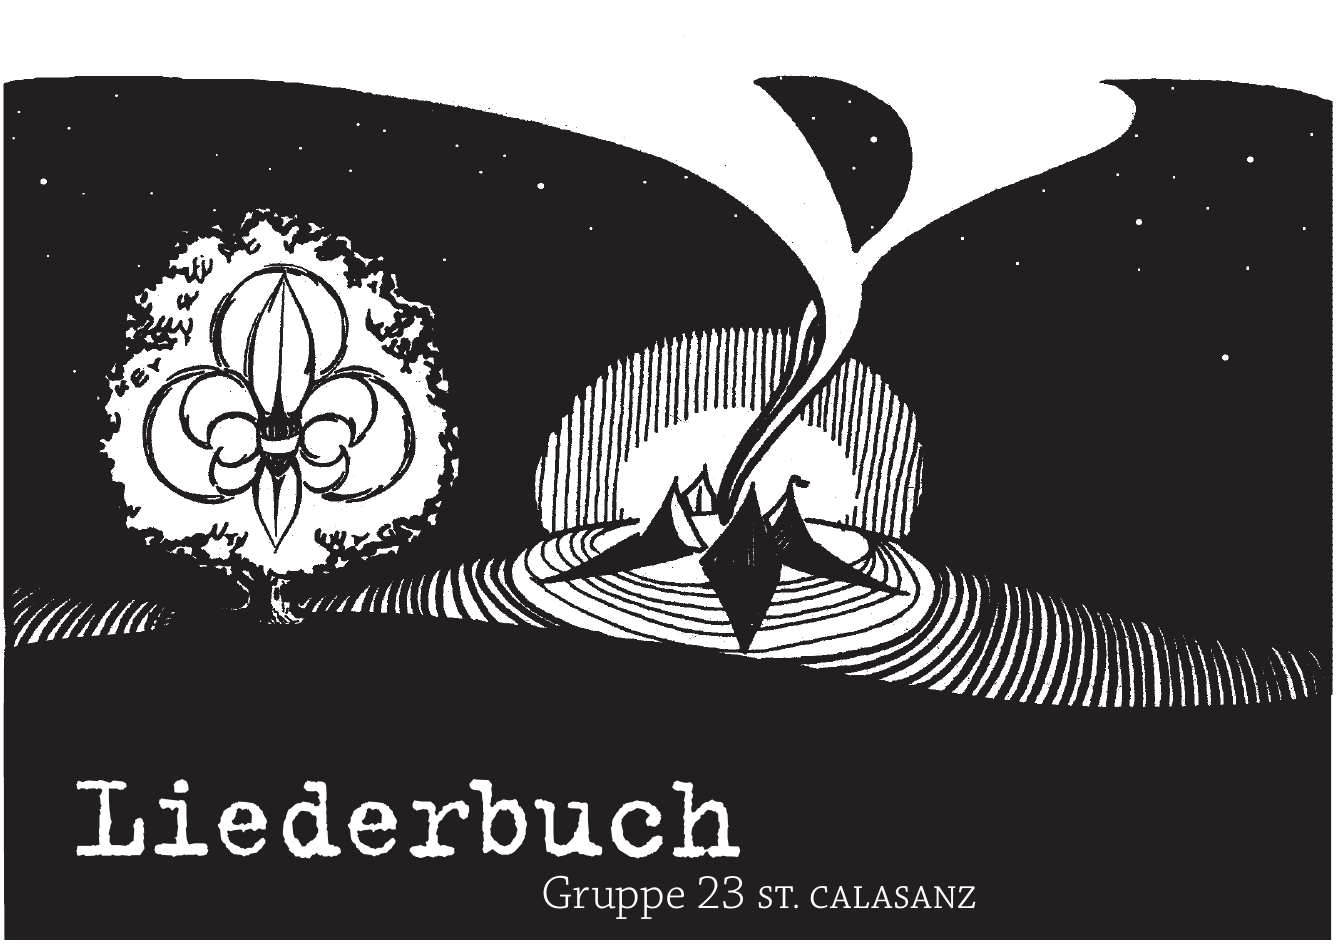
\includegraphics[scale=0.5]{titelblatt}
	\end{figure}
	\clearpage
	\pagestyle{fancy}
	
%	\tableofcontents


\begin{mybox}{\titlee{Blowing in the wind}}
	% Verse
	\begin{enumerate}
%		\item
%		\leavevmode%
%		\adjustbox{valign=t}{%
		\myverse{
			\acc{C} How many \acc{F} roads must a \acc{C} man walk \acc{Am} \\
			down, \acc{C} before you \acc{F} call him a \acc{C} man \acc{G7}? \\         
			\acc{C} How many \acc{F} seas must a \acc{C} white dove \acc{Am}  sail, \\                       
			\acc{C} before she \acc{F} sleeps in the \acc{G7} sand? \\                                
			Yes and \acc{C} how many \acc{F} times must the \\                                                                                                   
			\acc{C} cannon balls \acc{Am}  fly, \acc{C} before they’re \acc{F} forever \\
			\acc{G} banned \acc{G7}?
		}
		
		% Refrain
		\myrefrain{Refrain:}{The \acc{F} answer my \acc{G7} friend \\
		is \acc{C} blowing in the \acc{Am}  wind \\
		The \acc{F} answer is \acc{G7} blowing in the \acc{C} wind}
		
		\item
		\leavevmode%
		\adjustbox{valign=t}{%
		\begin{verses} 
			\acc{C} How many \acc{F} years can a \acc{C} mountain \acc{Am}  exist, \\
			\acc{C} before it is \acc{F} washed to the \acc{C} sea \acc{G7}? \\    
			Yes and \acc{C} how many \acc{F} years must some \acc{C} \\    
			people \acc{Am}  exist, \acc{C} before they’re \acc{F} allowed to \\
			be \acc{G7} free? \\
			Yes and \acc{C} how many \acc{F} times can a \acc{C} man \\
			turn his \acc{Am}  head, \acc{C} pretending that he \acc{F} just \\
			doesn’t \acc{G} see \acc{G7}? \Reff
		\end{verses}}
%		\pagebreak
		\item
		\leavevmode%
		\adjustbox{valign=t}{%
		\begin{verses} 
			Yes and \acc{C} how many \acc{F} times must a \acc{C} man \\
			look \acc{Am}  up, \acc{C} before he can \acc{F} see the \acc{C} sky \acc{G7}? \\
			Yes and \acc{C} how many \acc{F} ears must \acc{C} one man \acc{Am} \\
			have, \acc{C} before he can \acc{F} hear people \acc{G7} cry? \\
			Yes and \acc{C} how many \acc{F} deaths will it \acc{C} take till \\
			he \acc{Am}  knows, \acc{C} that too many \acc{F} people have \acc{G} \\
			died \acc{G7}? \Reff
		\end{verses}}
	\end{enumerate}
\end{mybox}

\begin{finalbox}{}
	\titlee{Blowing in the wind}
\end{finalbox}
% Verse
\begin{enumerate}
%		\item
%		\leavevmode%
%		\adjustbox{valign=t}{%
		\myverse{
			\acc{C} How many \acc{F} roads must a \acc{C} man walk \acc{Am} \\
			down, \acc{C} before you \acc{F} call him a \acc{C} man \acc{G7}? \\         
			\acc{C} How many \acc{F} seas must a \acc{C} white dove \acc{Am}  sail, \\                       
			\acc{C} before she \acc{F} sleeps in the \acc{G7} sand? \\                                
			Yes and \acc{C} how many \acc{F} times must the \\                                                                                                   
			\acc{C} cannon balls \acc{Am}  fly, \acc{C} before they’re \acc{F} forever \\
			\acc{G} banned \acc{G7}?
		}
		
		% Refrain
		\myrefrain{Refrain:}{The \acc{F} answer my \acc{G7} friend \\
			is \acc{C} blowing in the \acc{Am}  wind \\
			The \acc{F} answer is \acc{G7} blowing in the \acc{C} wind}
		
		\item
		\leavevmode%
		\adjustbox{valign=t}{%
			\begin{verses} 
				\acc{C} How many \acc{F} years can a \acc{C} mountain \acc{Am}  exist, \\
				\acc{C} before it is \acc{F} washed to the \acc{C} sea \acc{G7}? \\    
				Yes and \acc{C} how many \acc{F} years must some \acc{C} \\    
				people \acc{Am}  exist, \acc{C} before they’re \acc{F} allowed to \\
				be \acc{G7} free? \\
				Yes and \acc{C} how many \acc{F} times can a \acc{C} man \\
				turn his \acc{Am}  head, \acc{C} pretending that he \acc{F} just \\
				doesn’t \acc{G} see \acc{G7}? \Reff
		\end{verses}}
		%		\pagebreak
		\item
		\leavevmode%
		\adjustbox{valign=t}{%
			\begin{verses} 
				Yes and \acc{C} how many \acc{F} times must a \acc{C} man \\
				look \acc{Am}  up, \acc{C} before he can \acc{F} see the \acc{C} sky \acc{G7}? \\
				Yes and \acc{C} how many \acc{F} ears must \acc{C} one man \acc{Am} \\
				have, \acc{C} before he can \acc{F} hear people \acc{G7} cry? \\
				Yes and \acc{C} how many \acc{F} deaths will it \acc{C} take till \\
				he \acc{Am}  knows, \acc{C} that too many \acc{F} people have \acc{G} \\
				died \acc{G7}? \Reff
		\end{verses}}
	\end{enumerate}


\begin{finalbox2}{Nena}
	\titlee{Irgendwie, Irgendwo, Irgendwann}
\end{finalbox2}
% Verse
\begin{enumerate}
	\verse \acc{hm} Im Sturz durch Raum und \acc{F\#m} Zeit \\
	Richtung Unendlich-\acc{G}-keit \\
	\acc{hm} fliegen Motten in das \acc{F\#m} Licht \\
	genau wie du und \acc{G} ich. \acc{A} 
	
	\myrefrain{Refrain:}{\acc{Em} Irgendwie fängt irgend-\acc{C}-wann \\
	irgendwo die Zukunft \acc{D} an, \\
	ich warte nicht mehr \acc{G} lang. \\
	\acc{Em} Liebe wird aus Mut ge- \acc{C} -macht, \\
	denk nicht länger nach \\
	wir \acc{Am} fahr’n auf Feuerrädern \\
	Richtung \acc{D} Zukunft durch die Nacht \\
	\acc{Em} Gib mir die \acc{C} Hand, \\
	ich bau \acc{D} dir ein Schloß aus \acc{hm} Sand, \\
	irgend- \acc{C}-wie, irgend-\acc{G} -wo, irgend- \acc{D}-wann. \\
	\acc{Em} Die Zeit ist \acc{C} reif \\
	für ein biß- \acc{D}-chen Zärtlich-\acc{hm}-keit, \\
	irgend- \acc{C}-wie, irgend-\acc{G} -wo, irgend- \acc{D}-wann. }
	
	\myverse{\acc{hm} Im Sturz durch Zeit und \acc{F\#m} Raum \\
	erwacht aus einem \acc{G} Traum. \acc{D} \\
	\acc{hm} Nur ein kurzer Augen-\acc{F\#m}-blick, \\
	dann kehrt die Nacht zu-\acc{G}-rück. \acc{A} \Reff}
\end{enumerate}
%\end{mybox}

\clearpage
% ########################################	
	
{\centering\begin{tcolorbox}[hbox, enhanced, colback=white, bottom=1.5mm, left=0.5mm, right=1mm]
	\titlee{Blowing in the wind}
\end{tcolorbox}}

% Verse
\begin{enumerate}
	\verse \acc{C} How many \acc{F} roads must a \acc{C} man walk \acc{Am} \\
	down, \acc{C} before you \acc{F} call him a \acc{C} man \acc{G7}? \\         
	\acc{C} How many \acc{F} seas must a \acc{C} white dove \acc{Am}  sail, \\                       
	\acc{C} before she \acc{F} sleeps in the \acc{G7} sand? \\                                
	Yes and \acc{C} how many \acc{F} times must the \\                                                                                                   
	\acc{C} cannon balls \acc{Am}  fly, \acc{C} before they’re \acc{F} forever \\
	\acc{G} banned \acc{G7}?
	
	% Refrain
	\refrain{Refrain:}The \acc{F} answer my \acc{G7} friend \\
	is \acc{C} blowing in the \acc{Am}  wind \\
	The \acc{F} answer is \acc{G7} blowing in the \acc{C} wind
	
	\verse \acc{C} How many \acc{F} years can a \acc{C} mountain \acc{Am}  exist, \\
	\acc{C} before it is \acc{F} washed to the \acc{C} sea \acc{G7}? \\    
	Yes and \acc{C} how many \acc{F} years must some \acc{C} \\    
	people \acc{Am}  exist, \acc{C} before they’re \acc{F} allowed to \\
	be \acc{G7} free? \\
	Yes and \acc{C} how many \acc{F} times can a \acc{C} man \\
	turn his \acc{Am}  head, \acc{C} pretending that he \acc{F} just \\
	doesn’t \acc{G} see \acc{G7}? \Reff
	\pagebreak
	\verse  Yes and \acc{C} how many \acc{F} times must a \acc{C} man \\
	look \acc{Am}  up, \acc{C} before he can \acc{F} see the \acc{C} sky \acc{G7}? \\
	Yes and \acc{C} how many \acc{F} ears must \acc{C} one man \acc{Am} \\
	have, \acc{C} before he can \acc{F} hear people \acc{G7} cry? \\
	Yes and \acc{C} how many \acc{F} deaths will it \acc{C} take till \\
	he \acc{Am}  knows, \acc{C} that too many \acc{F} people have \acc{G} \\
	died \acc{G7}? \Reff \\[5mm]
\end{enumerate}

% Title
{\centering\begin{tcolorbox}[hbox, enhanced, colback=white, bottom=1.5mm, left=0.5mm, right=1mm]
	\titlee{Irgendwie, Irgendwo, Irgendwann}
\end{tcolorbox}}

% Verse
\begin{enumerate}
	\myverse{\acc{hm} Im Sturz durch Raum und \acc{F\#m} Zeit \\
	Richtung Unendlich-\acc{G}-keit \\
	\acc{hm} fliegen Motten in das \acc{F\#m} Licht \\
	genau wie du und \acc{G} ich. \acc{A} }
	
	\myrefrain{Refrain:}{\acc{Em} Irgendwie fängt irgend-\acc{C}-wann \\
	irgendwo die Zukunft \acc{D} an, \\
	ich warte nicht mehr \acc{G} lang. \\
	\acc{Em} Liebe wird aus Mut ge- \acc{C} -macht, \\
	denk nicht länger nach \\
	wir \acc{Am} fahr’n auf Feuerrädern \\
	Richtung \acc{D} Zukunft durch die Nacht \\
	\acc{Em} Gib mir die \acc{C} Hand, \\
	ich bau \acc{D} dir ein Schloß aus \acc{hm} Sand, \\
	irgend- \acc{C}-wie, irgend-\acc{G} -wo, irgend- \acc{D}-wann. \\
	\acc{Em} Die Zeit ist \acc{C} reif \\
	für ein biß- \acc{D}-chen Zärtlich-\acc{hm}-keit, \\
	irgend- \acc{C}-wie, irgend-\acc{G} -wo, irgend- \acc{D}-wann. }
	
	\verse \acc{hm} Im Sturz durch Zeit und \acc{F\#m} Raum \\
	erwacht aus einem \acc{G} Traum. \acc{D} \\
	\acc{hm} Nur ein kurzer Augen-\acc{F\#m}-blick, \\
	dann kehrt die Nacht zu-\acc{G}-rück. \acc{A} \Reff
\end{enumerate} 

\clearpage
% ########################################

% !TeX root = Liederbuchtest.tex

\myinput[]{Bruder Jakob}
\myinput[]{Gin-gan-gulli-gulli}
\myinput[Nena]{99 Luftballons}
\myinput[]{Father and Son}
\myinput[]{Die Hobelbank}
\myinput[]{Blowing in the Wind}
\myinput[]{Five hindred miles}
\myinput[]{Lady in Black}
\myinput[]{Auh, auh, die Nacht ist unser}
\myinput[Nena]{Irgendwie, Irgendwo, Irgendwann}
\myinput[]{Donna, Donna}
\myinput[]{Der Lagerboogie}
\myinput[]{American Pie}
\myinput[]{Ever sperm is sacred}
\myinput[Solalied 1992, Strechov, CSFR]{DamDam}
\myinput[]{With a little help from my friends}
\myinput[]{Ein belegtes Brot mit Schinken}
\myinput[The Beatles]{Hey Jude}
\myinput[]{Die Affen rasen durch den Wald}
\myinput[]{Wir vom Pfad}
\myinput[]{Franziskus}
\myinput[]{Drei Chinesen mit dem Kontrabass}
\myinput[]{Always look on the bright side}
\myinput[ABBA]{Fernando}
\myinput[]{Das Stachelschwein}
\myinput[]{Die Tante aus Marokko}
\myinput[Wham!]{Wonderwall}


\cleardoublepage
% toc
\toctitle{\faHashtag} 
\hyperlink{page.7}{99 Luftballons \textbf {7}} \\ 
\toctitle{B} 
\hyperlink{page.2}{Blowing in the wind \textbf {2}} \\ 
\hyperlink{page.4}{Blowing in the wind \textbf {4}} \\ 
\hyperlink{page.6}{Blowing in the wind \textbf {6}} \\ 
\toctitle{I} 
\hyperlink{page.2}{Irgendwie, Irgendwo, Irgendwann \textbf {2}} \\ 
\hyperlink{page.4}{Irgendwie, Irgendwo, Irgendwann \textbf {4}} \\ 
\hyperlink{page.6}{Irgendwie, Irgendwo, Irgendwann \textbf {6}} \\ 
\toctitle{W} 
\hyperlink{page.7}{Wir vom Pfad \textbf {7}} \\ 

\end{document}  

